%\documentclass[pdftex,12pt,a4paper]{report}
\documentclass[12pt]{article}

\usepackage[pdftex]{graphicx}

\usepackage{setspace}
\usepackage{scrextend}

\usepackage{amsmath}
\usepackage{amssymb}
\usepackage{mathtools}
\DeclarePairedDelimiter\ceil{\lceil}{\rceil}
\DeclarePairedDelimiter\floor{\lfloor}{\rfloor}
\usepackage[mathscr]{euscript}

\usepackage{longtable}
\usepackage{booktabs}
\usepackage{graphicx}
\usepackage{enumerate}
\usepackage[export]{adjustbox}
\usepackage[hidelinks]{hyperref}
\usepackage{url}
\usepackage{rotating}
\usepackage[labelfont=bf]{caption}
\usepackage{listings}
\newcommand{\sbt}{\,\begin{picture}(-1,1)(-1,-3)\circle*{3}\end{picture}\  }

\usepackage{color}

\definecolor{dkgreen}{rgb}{0,0.6,0}
\definecolor{gray}{rgb}{0.5,0.5,0.5}
\definecolor{mauve}{rgb}{0.58,0,0.82}

\lstset{frame=tb,
  language=Python,
  aboveskip=3mm,
  belowskip=3mm,
  showstringspaces=false,
  columns=flexible,
  basicstyle={\small\ttfamily},
  numbers=none,
  %numberstyle=\tiny\color{gray},
  %keywordstyle=\color{blue},
  %commentstyle=\color{dkgreen},
  %stringstyle=\color{mauve},
  breaklines=true,
  breakatwhitespace=true
  tabsize=3
}

%\lstdefinestyle{customc}{
%  belowcaptionskip=1\baselineskip,
%  breaklines=true,
%  frame=L,
%  xleftmargin=\parindent,
%  language=C,
%  showstringspaces=false,
%  basicstyle=\footnotesize\ttfamily,
%  keywordstyle=\bfseries\color{blue},
%  commentstyle=\itshape\color{purple},
%  identifierstyle=\color{black},
%  stringstyle=\color{orange},
%}
%\lstdefinestyle{customasm}{
%  belowcaptionskip=1\baselineskip,
%  frame=L,
%  xleftmargin=\parindent,
%  language=[x86masm]Assembler,
%  basicstyle=\footnotesize\ttfamily,
%  commentstyle=\itshape\color{purple!40!black},
%}

%\lstset{escapechar=@,style=customc}

\renewenvironment{description}[1][0em]
  {\list{}{\labelwidth=0pt \leftmargin=#1
   \let\makelabel\descriptionlabel}}
  {\endlist}
%\usepackage{enumitem}
%\setdescription{leftmargin=\parindent,labelindent=\parindent}

% adjust sections style and size
\usepackage{sectsty}

\usepackage{anysize}
\marginsize{2.5cm}{2.5cm}{1.3cm}{1.3cm}

% font commands for reference
%\it - italics typeface
%\sl - slanted typeface
%\bf - boldface typeface
%\sf - san serif typeface
%\tt - typewriter typeface
%\rm - normal (roman) typeface
%\em - roman or italics typeface
%\large - bigger type
%\Large - even bigger type
%\small - smaller type
%\normalsize - normal size

% line spacing options
%\singlespacing
%\onehalfspacing
%\doublespacing
\setstretch{1.2} % for custom spacing

%sets the paragraph indent
\setlength{\parindent}{1.5em}

% set the itemize indent
%\setitemize[0]{itemindent=-.7em}
% set the enumerate indent
%\setenumerate[0]{itemindent=-1.2em}

% new command \sbt for small button
%\renewcommand{\itemizei}{$\vcenter{\hbox{\tiny$\bullet$}}$}

%\newcommand{\HRule}{\rule{\linewidth}{0.5mm}}
%\newcommand{\Hrule}{\rule{\linewidth}{0.3mm}}

% texpos setup for placing text or images anywhere on the page
\usepackage[absolute]{textpos}
\setlength{\TPHorizModule}{30mm}
\setlength{\TPVertModule}{\TPHorizModule}
\textblockorigin{10mm}{10mm} % start everything near the top-left corner

\usepackage{libertine} \usepackage[libertine]{newtxmath}

\begin{document}
\begin{titlepage}
\begin{center}

\rule{\linewidth}{0.5mm}

\textsc{\large CIS 510 Final Project}
~\\[1cm]

{\Huge
	\textsc{Distributed Partial Differential \\\vspace{-.2em} Equation Solver For \\\vspace{.3em} 3-Dimensional Models}
}

\vspace{10pt}

\textsc{\Large (diffyq)}

\rule{\linewidth}{0.5mm}

\vfill

\textbf{Project Team:}\\
Adam Martini\\
Wes Erickson\\
Ran Tian\\

\vfill
{\large \today}

\end{center}
\end{titlepage}

\section*{Executive Summary}
We will design a flexible system for solving large partial differential equations in a parallel distributed system.  The product of our this project will solve 3-Dimensional models of any size for a given number of time steps.  Our system will take any size model and process it efficiently in parallel on multiple nodes.

%TODO: Breif description of the motivations for this project and why we need to use a distributed parallel processing model...

\chapter*{Project Description}
Anti-Kinetic Weapon Defense System (AKWDS) is the control software solution to integrate Flying Object Sensor Array (FOSA) and Ballistic Defense System (BDS). In some respects, the project can be thought of much like an automated Missle Command, Artillery, or Worms game. FOSA displays the data in a machine readable format. AKWDS houses the AI that makes decisions from the data. BDS actions the AKWDS firing command. FOSA and BDS for this project are backed by a basic physics simulation. We also plan to have FOSA output go to a 3D visualization in realtime or as a post-hoc analysis.

Simulation is planned to have 1 second between clock ticks. AKWDS processing time will be handled as a constant amount of delay or by rounding up the wall clock time to the nearest second. We simulate 1 second of delay between FOSA and AKWDS. 30 seconds of delay is simulated between AKWDS and BDS (simulating the time to move the firing mechanism). 60 seconds must elapse between shots.

We will write the n-body simulator, which will produce the FOSA stream and consume the BDS stream. We will also write AKWDS, which will consume the FOSA stream and produce a BDS stream. The simulator and AKWDS will live in separate process spaces and will be connected via TCP or MPI or some other IPC mechanism. We also plan to provide a 3D visualization using some visualization technology which may be online or posthoc (OpenGL, pov-ray, JavaFX, blender, VisIt, ???).


\section{Highlevel Architecture}
\label{architecture}

\begin{figure}[h]
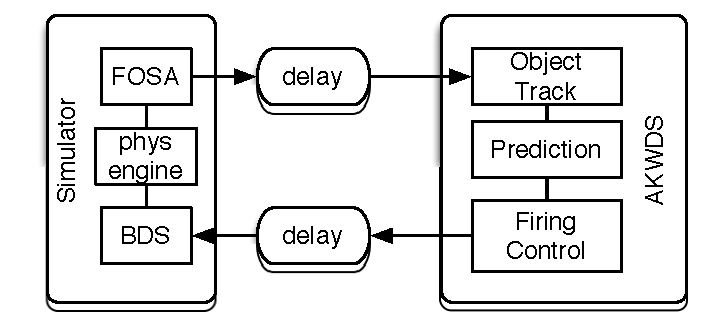
\includegraphics{./akwds_arch.pdf}
\caption{High Level Architecture Diagram}
\label{fig:arch}
\end{figure}

Figure 1 shows a block level diagram of the AKWDS software (without the visualization component). There are two main programs in the solution.
\begin{description}
\item[AKWDS] This is the control software that OSNAP needs in support of its mission to plan for and execute plans related to real and imagined extraterrestrial encounters. In this case, a hostile invasion scenario.
\item[Simulator] The Simulator is responsible for emulating the world that a deployed AKWDS system would be deployed in. This software supports evaluation and tuning of AKWDS without enduring actual extraterrestrial invasion.
\end{description}
AKWDS and the Simulator will be connected over a network. The Simulator will be responsible for handling the effects of delay called out in the project description.

\subsection*{Simulator}
The core of the simulator is a basic physics simulation. This N-body simulation will track projectiles and vehicles within the world and apply basic Newtonian physics. The simulator will expose the current location of each simulated object at regular intervals as a list of 3D cartesian coordinates and object radii. This stream will be sent using the FOSA format. The simulator will also take in a stream of BDS actions and add projectiles to the simulation as appropriate. The simulator also enforces some sanity rules regarding object motion and provides some basic flight paths for UFOs.

\subsection*{AKWDS}
AKWDS will take the FOSA stream of object locations and attempt to formulate some tracking of the objects (object A with location $L$ last time step is at location $L'$ this time step). This will be used to help estimate the future location of the object so that targets can be lead correctly for firing. AKWDS will then select a set of object to fire at and set of cannons to fire from and send the needed information via the BDS stream.

\subsection*{Visualization}
Visualization is not a core component of the project deliverable. However AKWDS debugging and demonstration will be very difficult without providing some animation of the system behavior. A visualizer, online or post-hoc, that works from the FOSA stream will be provided to help validate the software.

\section{Parallel Plan}

The each stage of the project data flow includes several places to introduce and explore parallelism.

\begin{description}
\item[Simulation] PETSc...
\item[Machine Learning] Which algorithms and how...
\item[Visualization] Visit, paraview...

%\item[Data Reduction] Data reduction...
%\begin{enumerate}
%  \item Spacial subsampling
%  \item Temporal subsampling
%  \item Compression
%\end{enumerate}
\end{description}

%We plan to look at system scaling by varying the number of initial objects in the simulation and the number of cannons available. We intend to look at wall clock time to complete a fixed number of simulation steps. We also intend to look at latency between the FOSA transmission time and BDS receive time to see if pipelining provides a significant benefit.

%If we have extra time, we would like to explore using MPI to spread the simulator and AKWDS computations across nodes to increase the size of simulation that can be done in realtime.



\section{Project Schedule}

\begin{tabular}{c | l}
Week & Deliverable\\
\hline
5 & {Petsc PDE solver installed and running data runs, identify parallel classifiers and get them running on acciss. \\ 
6 & Get classifiers working on acciss and extend/create code based on prediction goals. \\ 
7 & Process initial Petsc ouput to identify best classifiers. \\ 
8 & \\
9 & \\
10 & \\
\end{tabular}

\end{document}